\chapter{Fault tolerance and consensus} \label{ch:faultToleranceandconsensus}

In a distributed system there is a need for nodes to automatically recover from technical failures or partitions. If a node fails, the rest of the system should continue to operate without disturbing the clients. This is called fault tolerance. When the node has been repaired, it should be able to rejoin the distributed system and have its state brought up-to-date with the rest of the nodes. We say that a system is in a consensual state when a majority of nodes have agreed on some final value. In this chapter we look at the topic of fault tolerance and how it can be archived using the Raft consensus algorithm in a distributed system.

\section{The basics of fault tolerance}

A major difference between centralized and distributed systems is that we can experience partial failures in a distributed one. Suddenly, nodes can malfunction or become inaccessible due to network partitions. This can lead to decreased usability for clients. Therefore a strategy needs to be in place that can handle these kinds of failures. Without such the decrease of the operating quality for users would be proportional to the seriousness of the failure. Before diving into what types of failures we may witness, it is important to understand what values we seek in a distributed system and how they differ from each-other.

\noindent \textbf{Availability}: Availability is the quality of being able to be used right away. It is defined as a probability that the system will be ready when users need it to be. For high-availability or mission-critical systems, we usually see an uptime around five nines, which means the system has a probability of 99.999\% to be ready when users call.

\noindent \textbf{Reliability}: Reliability is the quality of being trustworthy and be able to produce consistency in measurements, i.e. the system will run without failures. It is defined as a time interval instead of a instance in time. If a system has high availability but still crashes randomly at times, it is unreliable. If a system never crashes, but is often shut down due to maintenance at a specific time, it is reliable.

\noindent \textbf{Safety}: To archive safety in a system, nothing fatal can happen should the system experience a failure. We often see this in mission-critical systems, where even a brief outage can have severe consequences. This could be a space rocket or a power plant facility. In less crucial systems, safety may not play such a huge role.

\noindent \textbf{Maintainability}: Maintainability tells us how easy a failed system can be examined, repaired and have worn-out components replaced by newer ones. We often see a correlation between high maintainability and high availability. 

\noindent \textbf{Atomicity}: Finally, atomicity is the quality of a operation or transaction that is indivisible and irreducible. Either it completes fully or nothing happens at all. This correlates to safety and can be seen especially in banking systems, where a money transaction between two accounts often involves multiple system and must be reversible should something interfere.

\noindent A system is said to fail when it cannot meet its promises or is unable to perform its required function. Failures are sometimes caused by errors, but they do not have to lead to failures, however. The cause of an error is a fault, that is an incorrect step, process or definition in a software application which causes the system to perform in an unintended manner. An technical fault in a branch of code on a node could lead to it experiencing an error, which could make it crash during execution. If other parts of the system depend on this node, the error could lead to a system failures. To classify these we use the following terms:

\noindent \textbf{Crash failures} occur when a node suddenly halts, but was working fine up until that point. A physical action must be taken to bring the node back up. \textbf{Omission failures} occur when a node does not respond to a incoming request. The request can malformed or perhaps the node fail to generate a response. \textbf{Timing failures} happen when a node does not respond within a time limit, maybe due to network delay or excessive load. \textbf{Response failures} is when a node respond, but its response is incorrect or is out of step with the current state of the system. \textbf{Arbitrary failures} are random and can occur at any time. These can be hard to narrow-down and correct.

\noindent To gain fault tolerance in a distributed system, we should seek to mask the occurrence of failures from other processes and have a back-up plan ready (redundant nodes) in case they should happen. We should also implement self-stabilization, so that the system will converge towards a correct state, no matter the initial one. Consensus is the key to archive this.

\section{The consensus problem}

The consensus problem is a fundamental problem in computer science and multi-computing systems applications. It states, that multiple processes or nodes in a system must come to an agreement on a single value for computation. Real world examples include transactions, clock synchronization and leader-election. Processes in a distributed system must talk to each-other, share their current state and somehow agree on one value, however this operation can be troublesome, as communications between nodes may fail or be unreliable in other ways, so we must define a consensus protocol that takes this into account. One way to go about it is to have the processes agree on a majority value, which requires at least one more than half the nodes in a system to reach consensus. This approach is straight-forward if we assume that the processes cannot fail. Every process $p_i$ begins in a \textit{undecided} state and proposes a single value $v_i$ from a set of values $V$ (i= 1, 2 ..., N). Each process then broadcasts this value to fellow processes and collect their values. When it has collected all \textbf{N} values and put them in a set $C$ it decides on the value $d_i$ that occurs the majority of times in the collected set $C$ hereby entering a \textit{decided} state, where it can no longer change $d_i$. To tolerate failures occurring, the protocol must have these properties:

\noindent \textbf{Termination:} Every process eventually decides on a value $d_i$.

\noindent \textbf{Agreement:} All processes must agree on the same decision value $d_i$.

\noindent \textbf{Integrity:} If all correct processes propose the same value $v_i$, then all correct processes will decide $v_i$ as $d_i$.

\noindent Now, if we assume that process $p_i$ can crash at arbitrary times during this consensus vote or become malicious, the process could potentially communicate wrong values to others hindering a consensus. This phenomenon is known as the Byzantine Generals Problem\footnote{\cite{Lamport1982}}. Next we look at the Raft consensus algorithm protocol, that provides a template for fault-tolerant and reliable consensus negotiation among processes.

\section{The Raft consensus algorithm}

Raft was proposed by Diego Ongaro and John Ousterhout in 2014. The goal was to offer a easy to understand, implementable and fault-tolerant consensus protocol to be used in a distributed system to replicate state machines. Raft works by managing a replicated log across multiple nodes and upholds simplicity by separating key elements of the process, that is leader election, log distribution and safety, versus a protocol like Paxos that has proven difficult to understand. Key features of Raft include:

\noindent \textbf{Strong leader:} The replication of log entries flow from the leader only. This simplifies log management, and enhances the leader role in Raft compared to other consensus protocols.

\noindent \textbf{Leader election:} From the start of the algorithm a leader has to be elected. Raft uses a randomized timer on each node to elect a leader. This is done to avoid conflicts and assumes all nodes are equally capable of being leaders. The time period electing a leader is called a term, and a new leader must be elected, if the old one fail.

\noindent \textbf{Membership changes:} Raft offers a join and leave command to dynamically change the membership of nodes. This is facilited by what is called a \textit{joint consensus} mechanism, that allows two different configurations to overlap while the transition is ongoing.

\noindent \textbf{Log replication:} The leader is responsible for replicating a log containing state information. During a term, client nodes (followers) send commands to the leader, and these are saved in a log. Upon replication, followers append the entries received from the leader in their own log. When a majority of followers have received the log, a leader adds it to his own state machine and it is then considered committed.

\noindent \textbf{Safety:} Only one leader can be elected for a given term. To ensure consistency, if a server has applied one log entry for an index in its log, then no other server can may apply a different value for the same index. Only a server with the newest log can become leader.

\noindent We will now look at the fundamentals for the protocol. We assume a cluster of five nodes ($N_1$ to $N_5$) participating in our Raft consensus algorithm. All nodes have a randomized timer $T_i$ = (i=1,2...,N).

\begin{figure}[H]
	\centering
	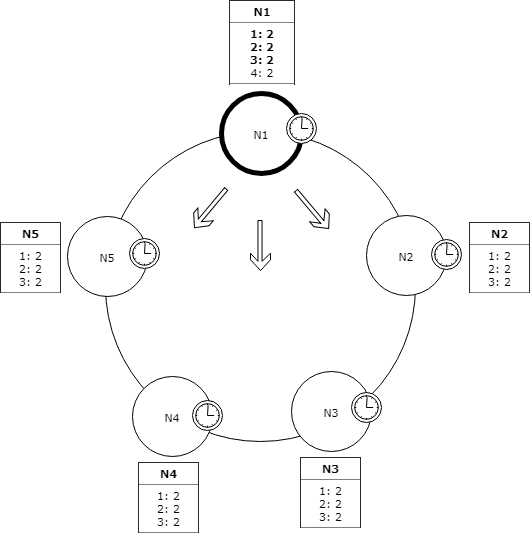
\includegraphics[scale=0.5]{faultTolerance/fig/Raft.png}
	\caption{The topology for our Raft setup. N1 is leader and replicates its state log to follower nodes.}
	\label{fig:raft}
\end{figure}


